
\subsection{Operational scenarios}\label{sec:opscenarios}
To study the different aspects of our predictions for the operation of the ITk strip system throughout its lifetime we performed the calculation of the system parameters over the expected 14 years of operation in monthly steps. Time-dependent inputs to the calculations were given from the expected performance of the LHC (figure~\ref{fig:opscenarios}a) and different profiles for the cooling temperature. We studied flat cooling temperature scenarios at different temperatures starting at -35$^\circ$C, the lowest evaporation temperature achievable with the ITk evaporative CO$_2$ cooling system, and a `ramp' scenario, where the cooling temperature starts at 0$^\circ$C and gradually is lowered down to -35$^\circ$C (figure~\ref{fig:opscenarios}b).

\begin{figure}[ht]
\centering
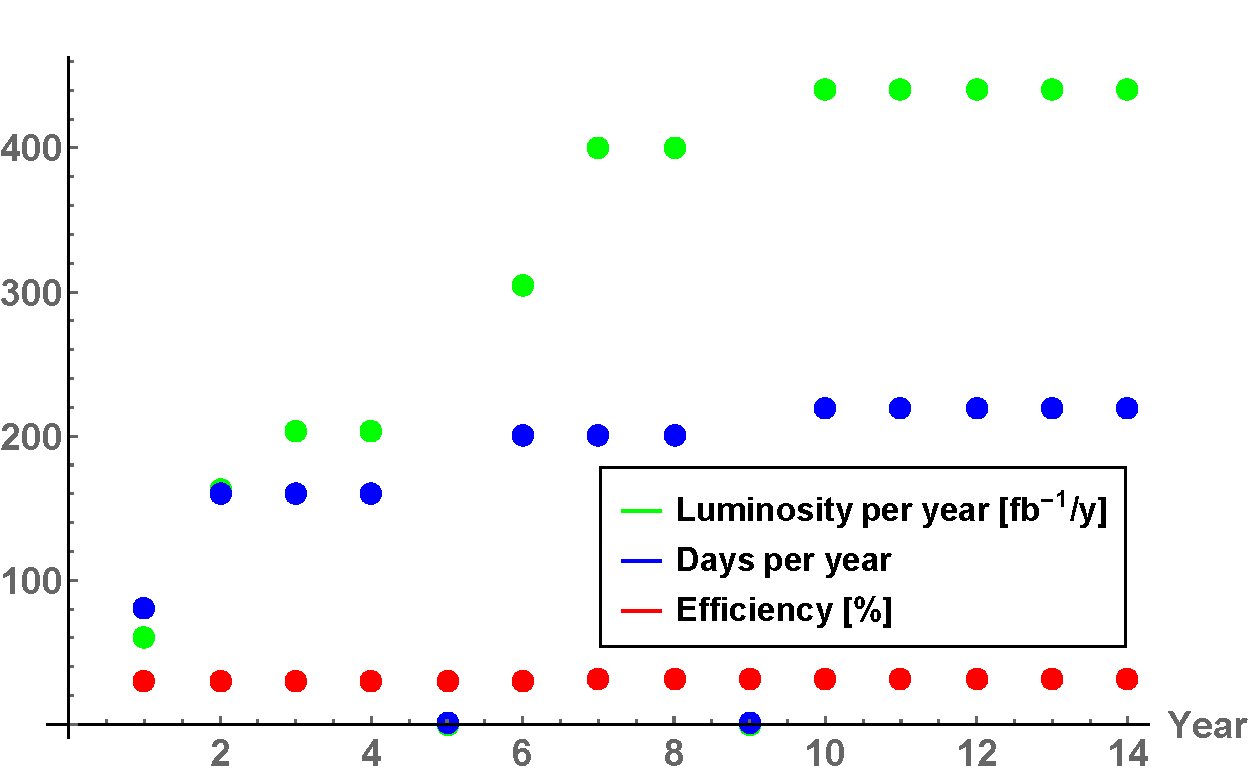
\includegraphics[width=0.4\linewidth]{figures/LHCperformance.pdf}\quad\quad
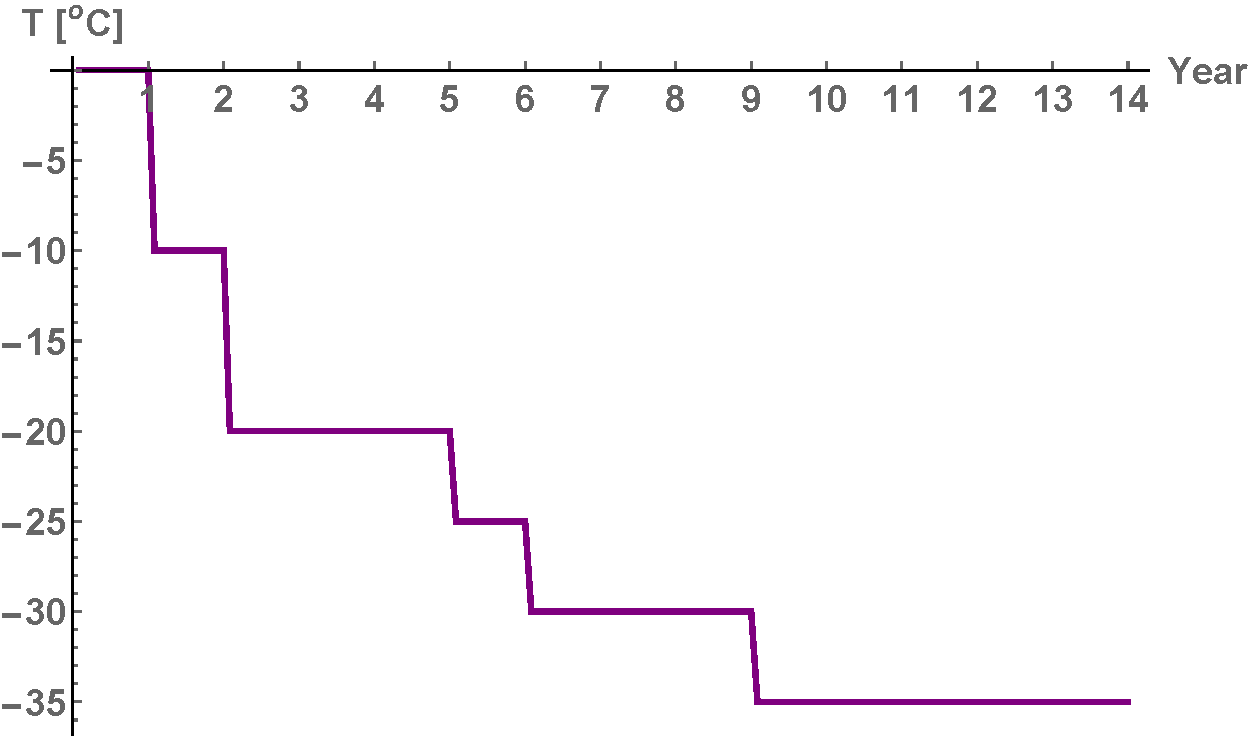
\includegraphics[width=0.4\linewidth]{figures/coolingramp.pdf}
\caption{Expected LHC performance (left) and cooling ramp' scenario for the cooling temperatures (right). Year-long shutdowns of the LHC are anticipated in years 5 and 9.}
\label{fig:opscenarios}
\end{figure}

\subsection{Safety factors}
To ensure the robustness of the system design against errors in the assumptions used in the model we ran the model in addition to the nominal set of input parameters with a set where some key inputs have been degraded. The set of safety factors used are given in table~\ref{tab:safetyfactors}. Each safety factor has been estimated individually based on experience, the complexity of the system aspect described by the parameter, and from available data or the absence of such data. Note that when the model was evaluated with safety factors all the safety factors in table~\ref{tab:safetyfactors} were used together, a situation which is unlikely to occur in the real system, thus providing a worst case estimate for the performance of the ITk strip system.

\begin{table}[htb]
\caption{Safety factors.}
\label{tab:safetyfactors}
\centering
\begin{tabular}{lcl}
Safety factor on & Value & Reason \\
\hline
Fluence  & 50\% & Accuracy of fluence calculations and uncertainties in material distributions\\
Thermal impedance & 10\% & Local support build tolerances\\
Digital current & 20\% & Final chip performance and parametrization of TID effect\\
Analog current & 5\% & Final chip performance\\
Tape impedance & 10\% & Electrical tape manufacturing tolerances\\
Bias voltage & 700~V & Increased bias voltage from 500~V to maintain S/N\\
\end{tabular}
\end{table}

\subsection{Results}
The thermo-electrical model provides a large range of predictions for the operation of the strip system. A detailed discussion of all results would only be of interest for ITk strip community members and is beyond the scope of this article. Instead we will present here a subset of results to demonstrate the capabilities and use of the thermo-electrical model for the design of the detector system.

\subsubsection{Module properties}

Some example output plots for module properties from the thermo-electrical modules are shown in figures~\ref{fig:moduleflatperformance} and~\ref{fig:modulerampperformance}. The different radiation-dependent effects occur on different times scales. The maximum in the digital chip power due to the TID effect occurs relatively early (in year 1 to 4), although the bump has a long tail, particularly in the outer layers of the barrel. The sensor leakage power on the other hand grows towards the end of the lifetime of the ITk. Due to the radius-dependence of the radiation environment the radiation-induced effects are most pronounced in the innermost layer.

\begin{figure}[ht]
\centering
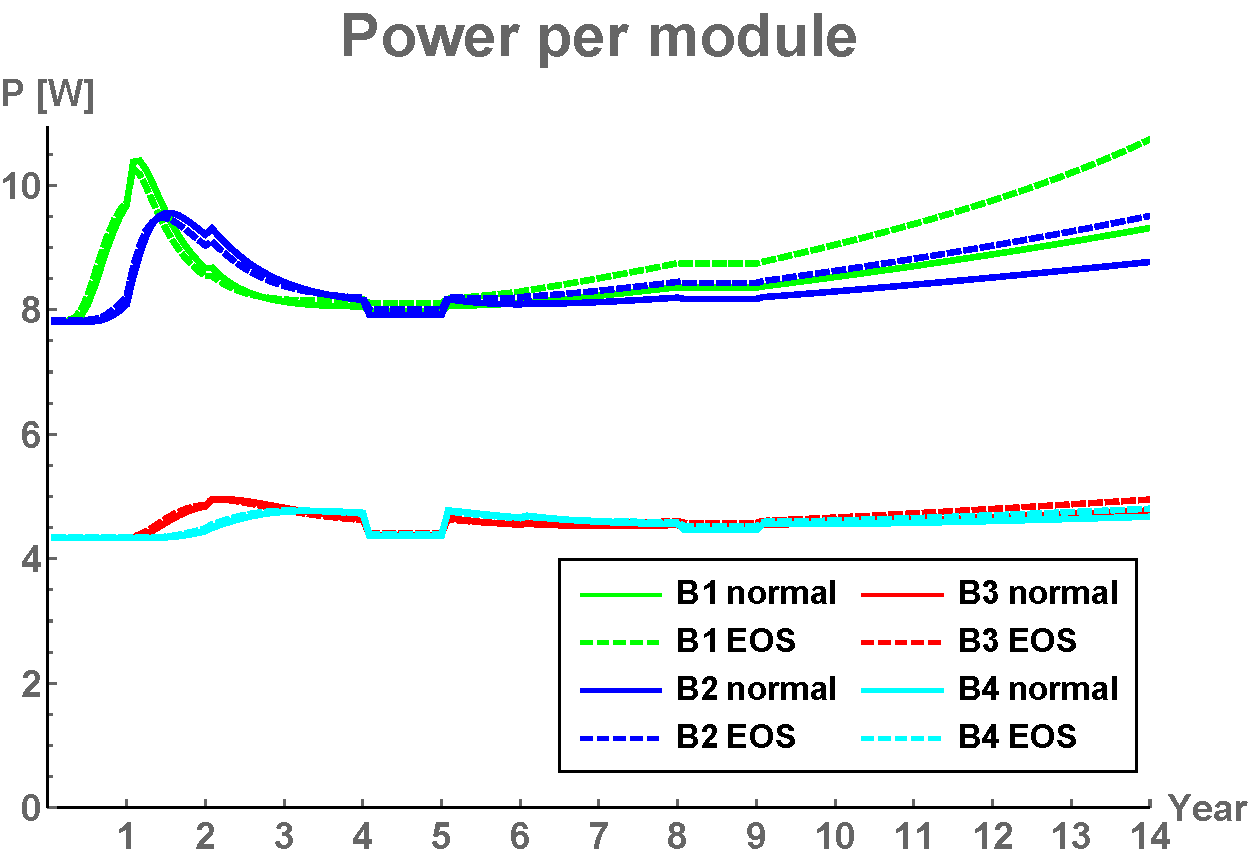
\includegraphics[width=0.4\linewidth]{figures/powerpermodule.pdf}\quad\quad
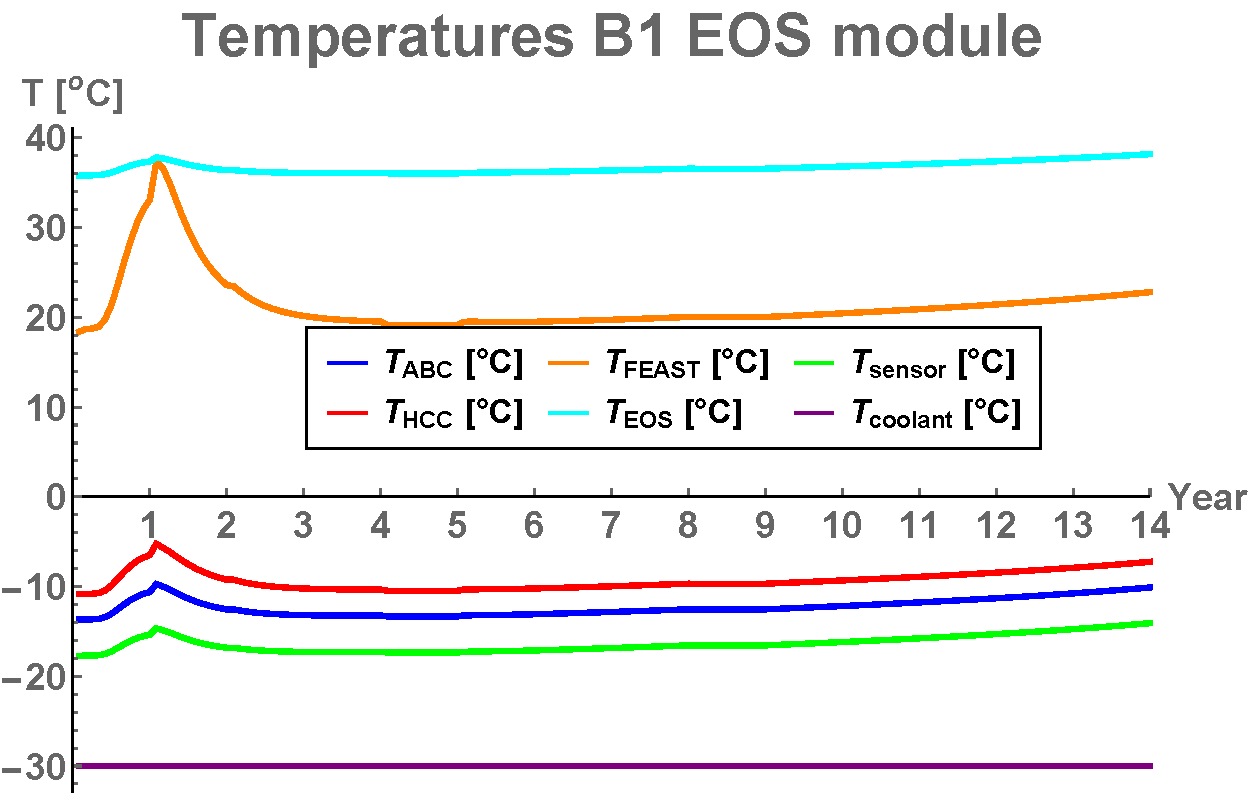
\includegraphics[width=0.4\linewidth]{figures/Teosmodule.pdf}
\caption{Examples for barrel module performance predictions for a flat cooling scenario (-30$^\circ$) including safety factors. Power per module (left). Temperatures for different parts of and end-of-stave barrel module in the innermost barrel (right).}
\label{fig:moduleflatperformance}
\end{figure}

\begin{figure}[ht]
\centering
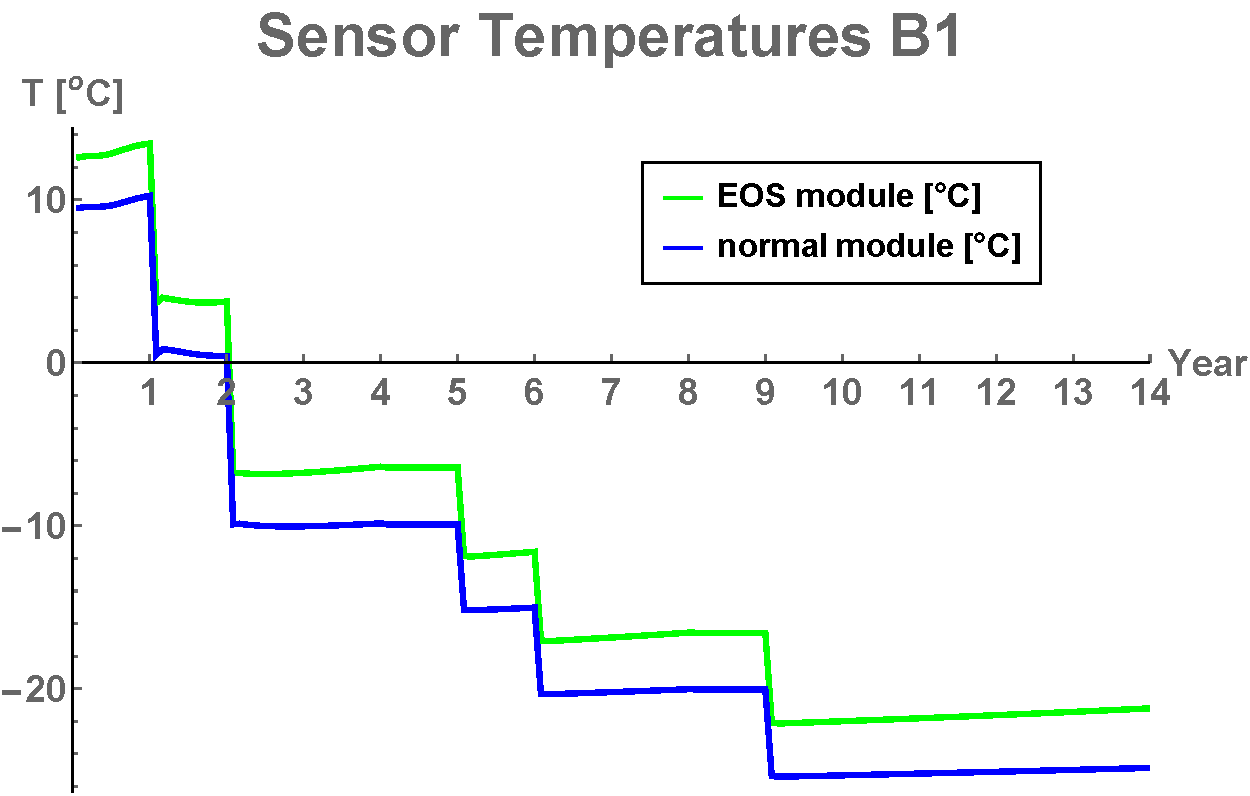
\includegraphics[width=0.4\linewidth]{figures/Tmodule.pdf}\quad\quad
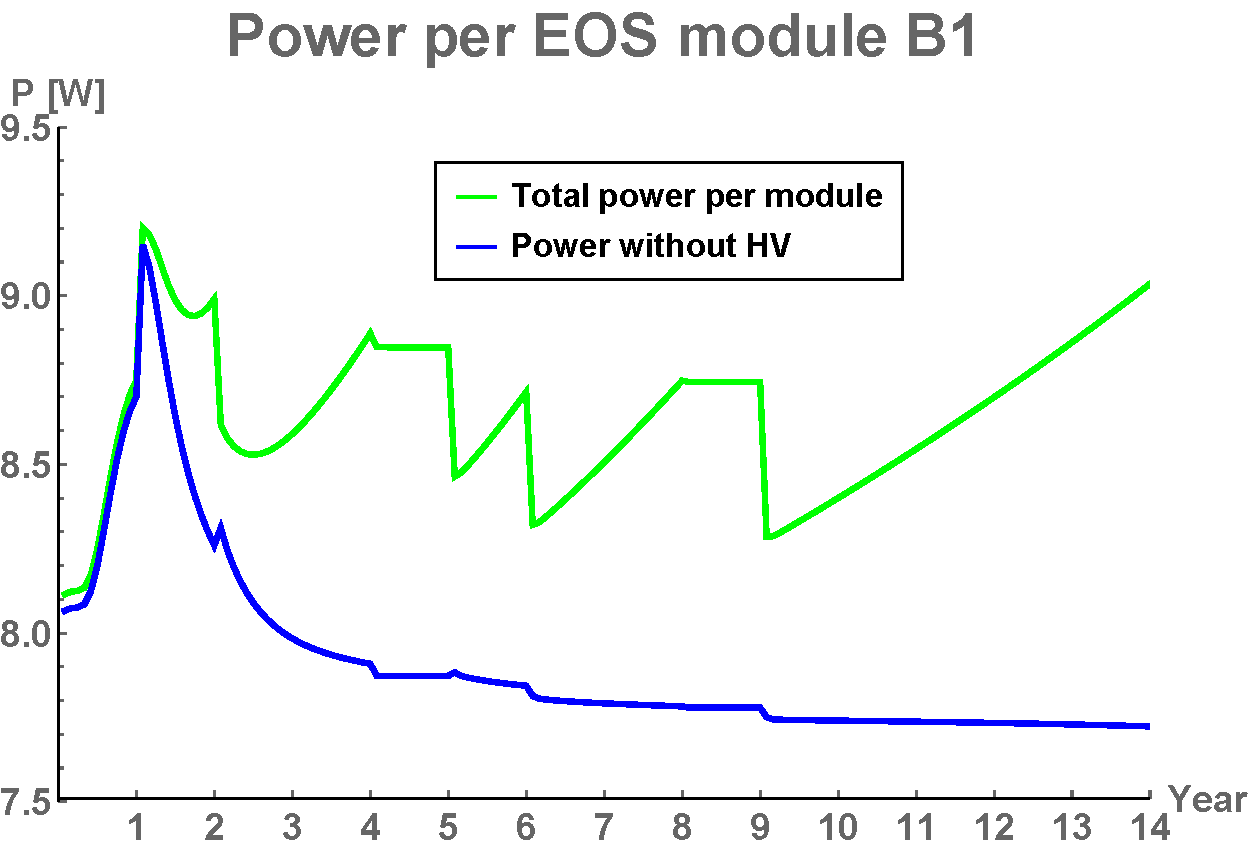
\includegraphics[width=0.4\linewidth]{figures/Peosmodule.pdf}
\caption{Examples for barrel module performance predictions for the ramp cooling scenario including safety factors. Temperature in innermost barrel modules (left). Power in an end-of-stave barrel module in the innermost barrel (right).}
\label{fig:modulerampperformance}
\end{figure}

\subsubsection{System properties}
One of the key concerns for the design of the strip system is thermal stability of the system. If the cooling temperature is too high to limit the leakage power from the radiation-damaged sensors to a level where it can still be removed the system is unstable (it goes into `thermal runaway'). In this case there is no solution to the set of equations in the thermo-electrical model any more and the numerical search for a solution fails. In the barrel strip system this happens in the last year of operation at a cooling temperature of -15$^\circ$C under nominal conditions, and at -25$^\circ$C (in year 13) with safety factors applied. As the design cooling temperature of the ITk cooling system is -35$^\circ$C we have confidence that the ITk strip system has sufficient margin for thermal stability.  

Beyond the issue of stability, the thermo-electrical model delivers predictions for the development of current and power requirements for the overall system. Some of the predictions are shown in figure~\ref{fig:systemperformance}. The Ignoring this time dependence could lead to overspecification of the cooling system.

\begin{figure}[ht]
\centering
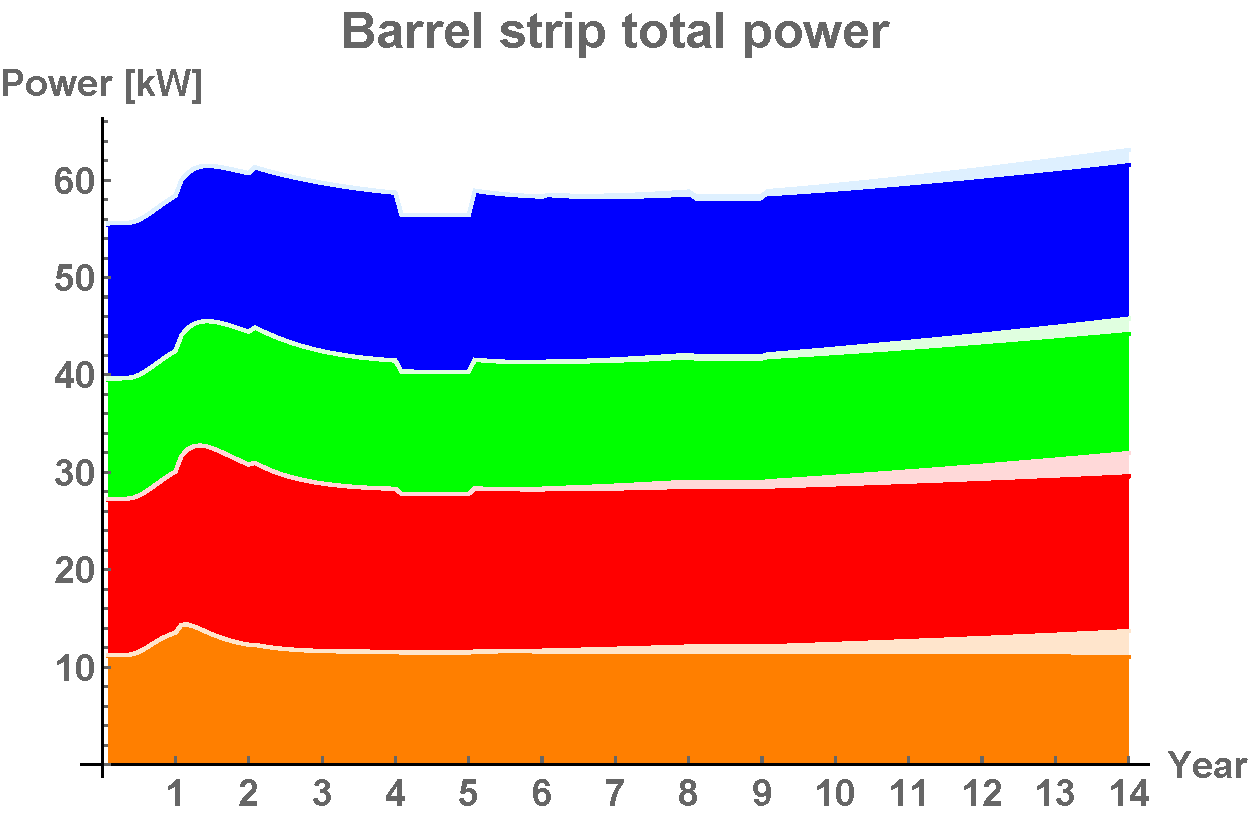
\includegraphics[width=0.4\linewidth]{figures/Totalbarrelpower-30.pdf}
\caption{Examples for system performance predictions. Barrel total power requirements for flat -30$^\circ$ cooling including safety factors (left): The plot shows the stacked power requirements for the four barrels (orange: innermost barrel, blue: outermost barrel). The greyed parts are contributions from HV power for the four barrels.}
\label{fig:systemperformance}
\end{figure}

These predictions are now used throughout the strip project to conistently size power supply and cooling systems. Including safety factors in the predictions gives us some confidence that the designs are robust and by using commonly agreed safety factors we ensure a consistent use of safety factors throughout the project and prevent safty factor creep.  

Because of the different timescales for the peak power due to the TID effect and the sensor leakage due to radiation there is room for the optimization of the cooling temperature profile for minimal power. The thermo-electrical model is a powerful tool to plan such an optimized cooling profile. In fact, the cooling `ramp' scenario introduced in section~\ref{sec:opscenarios} is the result of such an optimization (figure~\ref{fig:rampoptimization}).

\begin{figure}[ht]
\centering
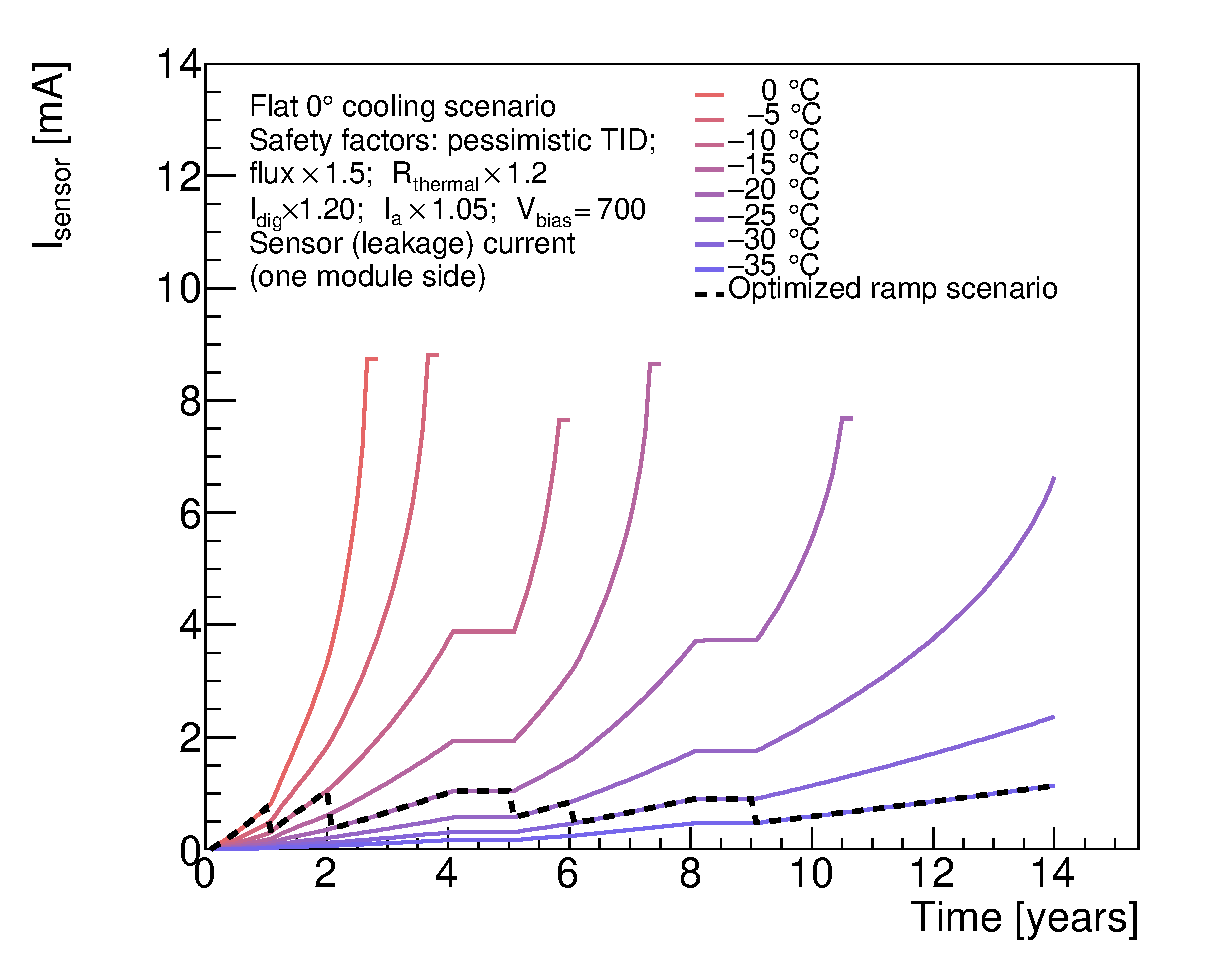
\includegraphics[width=0.49\linewidth]{figures/SensorCurrent_R3_newramp.eps}
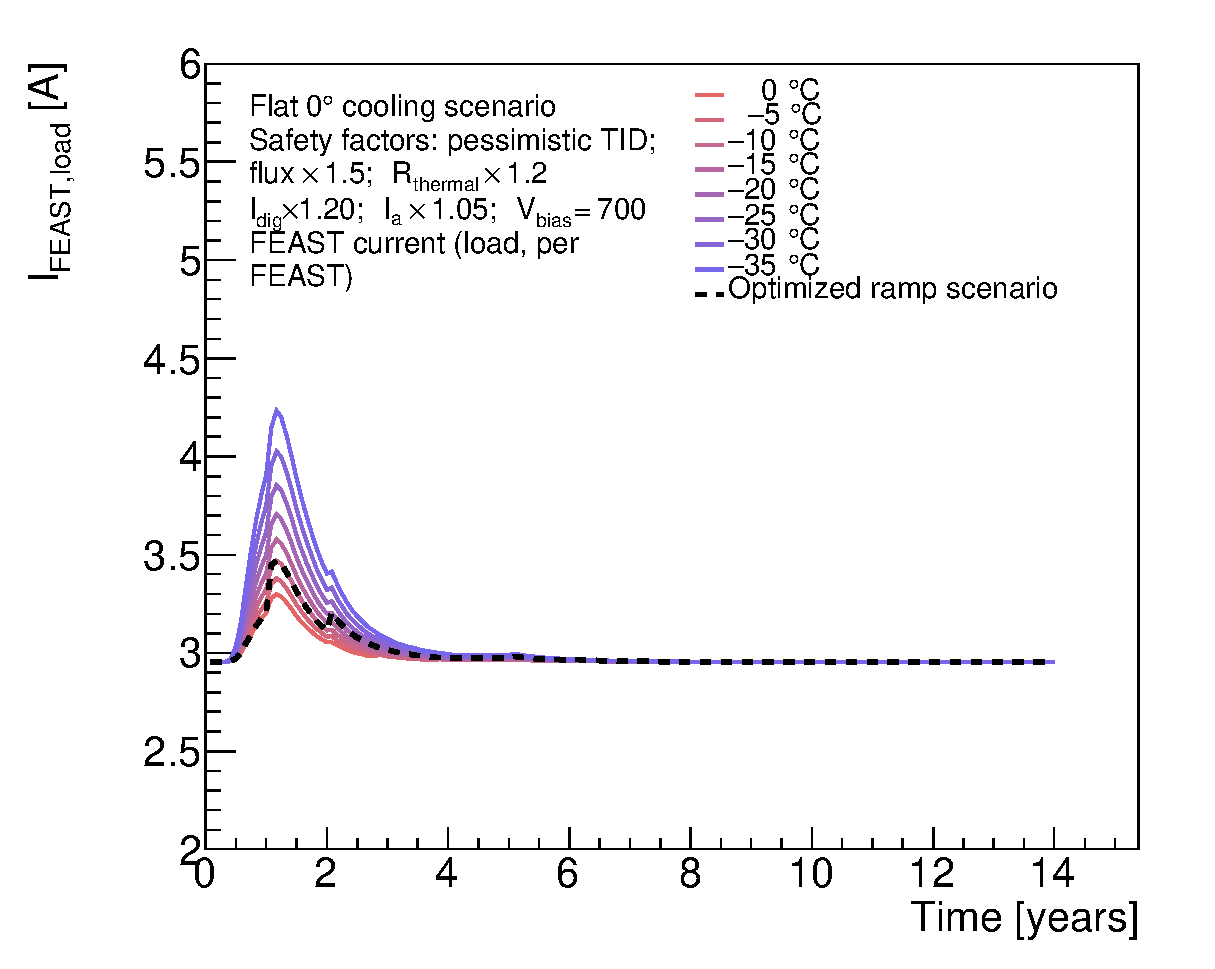
\includegraphics[width=0.49\linewidth]{figures/FeastCurrent_R1_newramp.eps}
\caption{Optimization of the cooling `ramp' scenario. The dashed lines represents the ramp scenario, which has been selected so that the sensor leakage current is stable throughout the lifetime of the ITk (left). The higher cooling temperatures in the first years keep the TID effect relatively small (right).}
\label{fig:rampoptimization}
\end{figure}
